\documentclass{epsrc}

%I use these routinely but may not be needed
\usepackage{chemstyle}
\usepackage[version=3]{mhchem}
\usepackage{graphicx}
\usepackage{amsmath}
\usepackage{amsfonts}
\usepackage{hyperref}
\usepackage{lipsum}

%required for wrapping text around figures
\usepackage{wrapfig}

%set up different captions
\usepackage{caption}
\captionsetup[figure]{labelfont={it,bf},textfont=it}

%set up two bibliographies for parts 1 and 2
\usepackage[resetlabels]{multibib}
\newcites{A,B}{References,%
References}

\usepackage[british]{babel}

%%%Fancy header settings. Remove draft parts for final
\usepackage{fancyhdr}
\setlength{\headheight}{20pt}
\pagestyle{fancy}
\rhead[]{Benedek et al. (2022)}
\lhead[]{Mitigating Joule Expansion in Multicell Atomic Quantum Memory}
\chead[]{}

\cfoot[\thepage]{\thepage}

\begin{document}

\title{Mitigating Joule Expansion in Multicell Atomic Quantum Memory}

\author{Prof. K. Benedek, et al}
\maketitle

\vspace{8pt}

\section{Abstract}

With the physical absence of scalable quantum information designs, the search for appropriate solutions continues. By drawing advances off recent work from colleagues \citeA{MainMAQM}, herein, we propose to utilise dipole trap arrays \citeA{OptTweezer} to house microensembles of 2D atomic memory cells for improving the memory lifespan of Multicell Atomic Quantum Memory (MAQM) repeaters. This effort forecasts an increase over the current state-of-the-art memory lifespan of 1ms \citeA{MainMAQM}, by up to three orders of magnitude\citeA{OptTweezer}. 

\part{Previous track record and expertise at the host institution}

The Department of Physics at the University of Strathclyde is a well-established and world-renowned centre of excellence in theoretical and experimental quantum optics and information. The team selected for this proposal is no exception, and each bring their own strengths to this project, as listed below.

\vspace{8pt}

\textbf{Prof. Kata Benedek} (KB) has completed her DPhil at the University of Oxford under the supervision of professor David Deutsch on "Lattice-based post-quantum cryptography" where she worked on numerically simulating and experimentally realising algorithms for the quantum era and their interoperation with existing classical protocols. After her doctorate she was a Pappalardo fellow at MIT's physics group where she demonstrated quantum logic in a cryogenic surface-electrode ion trap \citeA{MIT} amongst other projects. After her fellowship at MIT she joined Strathclyde's EQOP group as a Reader (now a full professor) to lead the effort towards scalable quantum communication hardware. 

\vspace{16pt}

\textbf{Dr. Lewis MacLeod Russell} (LR) has completed two EPSRC-funded post-doctoral fellowships, after defending his PhD thesis on the "Development of a dipole trap based atomic clock" under Prof. Erling Riis; all at the university's EQOP group. As Dr. Russell participated in similar quantum hardware projects funded from EPSRC grants \href{https://gow.epsrc.ukri.org/NGBOViewGrant.aspx?GrantRef=EP/M013294/1}{EP/M013294/1}, \href{https://gow.epsrc.ukri.org/NGBOViewGrant.aspx?GrantRef=EP/T001046/1}{EP/T001046/1}, \href{https://gow.epsrc.ukri.org/NGBOViewGrant.aspx?GrantRef=EP/P009565/1}{EP/P009565/1}, and \href{https://gow.epsrc.ukri.org/NGBOViewGrant.aspx?GrantRef=EP/T005386/1}{EP/T005386/1}, his expertise, which surrounds amongst others, the integration of quantum systems and information is directly transferable to the experiment.

\vspace{16pt}

\textbf{Dr. Christoforos Iakovou} (CI) completed his PhD on "Trapped ion quantum information" at ETH Zürich under the supervision of Jonathan Home. During his time at ETH he was involved in the design and execution of pioneering experiments using optical tweezers arrays for trapped ion quantum computing. Following his doctorate, Dr. Iakovou joined the team of Wenhui Li at NUS in Singapore as a postdoctoral fellow working on Rydberg atoms in optical lattices for quantum simulation. With a track record of 15 publications in peer-reviewed journals and more than 7 years of experience in optical traps for quantum information, experimental design, and vacuum technology, his experience is of high relevance to the proposed project.

\vspace{16pt}

\section{EPSRC Relevance}

This proposal addresses the EPSRC Themes of ``Physical Sciences", ``Quantum Technologies", and ``Information and Communication Technologies".

\vspace{16pt}

\section{Contribution to UK Competitiveness}

Success in our objectives will prove as a major step in the field of quantum communication. With the current EPSRC investment portfolio amounting to £150M towards Quantum Technologies, around 6\% of the total funding resources, the EPSRC's commitment towards the sustainable and long-term development of quantum technology is clear. In an ever evolving global landscape, it is vital that the UK maintains a significant capability in its research and development services; and with global advances in quantum research, the UK's quantum technology offerings are no exception. Our MAQM development is a vital component to this greater objective.  

A successful grant application will enable our team to continue our contributive efforts towards the UK's quantum capabilities; on a larger scale, this includes the development of large-scale quantum networks for the UK, ultimately leading to a quantum internet. Failure to create such networks carries the high-potential risk of seeing the UK out-competed by other countries as a scientific and information security service provider.

Our most notable research projects have included investigations into hybrid quantum memory from superconducting qubits \citeA{hybridquantum1}, as well as the realisation of an experimental 105-qubit quantum memory system \citeA{105qRAM}. The knowledge gained from these investigations highlights our ability to develop the proposed MAQM hardware.

\vspace{16pt}

\section{External Contributors}

Since demonstrating a successful quantum repeater based qRAM design in 2021 \citeA{MainMAQM}, Dr. Chang Li (CL) of Tsinghua University will provide us with primary assistance and insight on replicating the aforementioned qRAM scheme. This will then allow the Strathclyde team to adapt their proposed dipole trap configuration for longer qRAM lifetimes. 

Additionally, we call on the cooperation of visiting fellow Dr. Nils Hempler (NH) - General Manager of the quantum research and systems division of industrial stakeholder and partner M-Squared Lasers, based in Glasgow. He shall manage and facilitate the research and development on scaling and potentially commercialising a version of the proposed qRAM. 

\part{Description of proposed research and context}

\vspace{4pt}

\section{Introduction}

The realisation of quantum technologies is of transformative importance as it disrupts not only the way we think about information, it may also replace the entire classical computing infrastructure which is today prevalent. Their superior computational ability in certain tasks \citeA{deutsch1992rapid, shor1999polynomial}, grants the capability to break current data encryption algorithms \citeA{postQcrypto} and also offers greater computational disposal to future scientific research \citeA{atas20212,semeghini2021probing}. It has also been demonstrated that they are unrivaled in their security of end-to-end information exchange \citeA{PhysRevLett.85.441, PubKeyQcrypto}. Contrary to classical information theory where the most basic unit of information is the bit, depicted by zeroes and ones by electrical signals at two different levels for example, in the regime of quantum information the unit analog to the bit is the quantum-bit or "qubit". While a qubit can be a classical zero or one, because of quantum mechanical superposition, it can be also be in any linear combination state of these classical bits \citeA{nielsen2002quantum}. It has been demonstrated that by precisely manipulating certain systems, we can indeed engineer qubits in a variety of ways. Among others, some of the most notable have been the control of an electron's spin state in silicon, neutral atoms excited to Rydberg states and diamond nitrogen vacancies \citeA{pla2012single,levine2018high,liu2018quantum}. 

Furthermore, a set of routine tasks can be flawlessly executed classically, thanks to a temporary type of memory, the Random Access Memory (RAM). Such tasks, include the ability to copy, distribute, read and write streams of data. It constitutes a major leap in the field to invent quantum hardware with which reading and writing data is to be done in an effective manner. A way which this is to be done, is by demonstrating quantum-RAMs or "qRAMs". Correspondingly to RAM, qRAM is responsible for the retrieval of quantum states to be read at a later time. However as with classical components, engineering quantum hardware comes with its challenges. Effects which are present, like atomic free expansion, irreversibly expands the memory cell to an unreadable state and destroys the overall long-lived distributed entanglement\citeA{MainMAQM,zhang2020quantum,tabor1991gases}. Additionally, the no-cloning theorem\citeA{wootters1982single} prohibits the replication of arbitrary quantum states. Thus, various hardware design proposals for tackling the aforementioned challenges on storing and reading quantum information must be explored. 

Herein, we propose an experiment to realise a quantum repeater node based on multicell atomic quantum memory (MAQM) as demonstrated by Li et al. (2021), a co-author of this proposal and collaborator. By utilising optical tweezers arrays\citeA{Mie} to trap and manipulate atomic ensembles rather than magneto-optical traps (MOTs), this current design can be improved. Optical tweezers arrays, which use highly focused laser beams on microscopic atomic ensembles are promising candidates in increasing the memory lifetime of the memory cells by mitigating the atomic free expansion of the ensembles. This will result in longer lifetime per memory cell and entanglement between nodes is maintained for longer times. This will constitute an important step towards goals such as scalable quantum computing components and quantum networks for global scale quantum key distribution (QKD)\citeA{simon2017towards}.

\vspace{16pt}

\section{Strategic Objectives}

\vspace{4pt}

\begin{enumerate}
  \item Build the multicell atomic quantum memory (MAQM) experimental set-up with optical tweezers array trap.
  \item Achieve the current state-of-the-art memory lifetime of 1 ms.
  \item Surpass the current state-of-the-art lifetime by 2 - 3 order of magnitude, i.e., 0.1 – 1 second of memory lifetime.
  \item Participate in R\&D with M2Lasers industrial partner, investigating scalable solutions of MAQM for potential commercialisation.
  \item Organise international outreach workshops on quantum hardware with Chinese collaborators.
\end{enumerate}

\vspace{8pt}

Given the current infancy of quantum computing technologies, the industrial R\&D component of our objectives carries the risk of becoming irrelevant or out-dated; future designs for scalable and commercial quantum communication hardware are, of course, unknown. However, the scientific knowledge gained from the creation of our MAQM design is still of great importance to the further development of quantum memory hardware.

\vspace{16pt}

\section{Background} \label{Background}

\vspace{4pt}

\subsection{Optical Tweezers}

\begin{wrapfigure}{r}{0.5\textwidth}
\vspace{-11pt}
	\begin{center}
		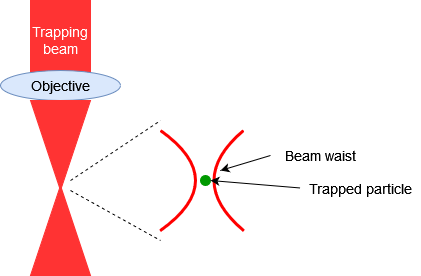
\includegraphics[width=8.2cm]{img/Tweezer.png}
			\vspace{-30pt}
		\caption{Optical Tweezer}
		\label{fig:tweez}
	\end{center}
\end{wrapfigure}

Optical tweezers - or optical dipole traps - are instruments that use highly focused laser beams to control and trap small particles. This method of particle manipulation has been presented first by Arthur Askin in 1997 \citeA{Ashkin} and has been increasingly used in physics and biological sciences \citeA{}.

A particle, which is placed in the path of a laser beam experiences optical forces, split into two components: a scattering force $F_S$, in the direction of propagation of the light, and a gradient force $F_G$ in the direction of the light gradient. For a stable trapping in the three dimensions, the force pulling the particle to the focused region must be greater than force $F_S$ that pushes it away. Therefore, a highly focused laser beam must be created. This focused region, of the highest gradient is called beam waist as shown on \ref{fig:tweez}.

For optical trapping, the size of the trapped particle, is considered and compared to the wavelength of the trapping light. If the particle diameter is much larger than the wavelength of the light, i.e. $a\gg\lambda$ condition for the "Mie regime" holds, and the forces acting on the particle can be calculated by using ray optics. When the diameter is comparable with the trapping wavelength, i.e. $a \sim \lambda$ complex electromagnetic field analysis is needed. In the case where the particle diameter is much smaller than the wavelength, i.e. $a\ll\lambda$ conditions for Rayleigh scattering are satisfied \citeA{Mie}.

We are proposing to experiment in the Rayleigh regime, where the trapped atom is considered as a point dipole in an inhomogeneous electromagnetic field. The scattering force experienced is owed to the absorption and re-radiation of light by the trapped atom:
\begin{equation}
    F_S=\frac{I_0 \sigma n_m}{c}
\end{equation}
Where $I_0$ is the intensity of the incident light, $\sigma$ is the cross-section of the sphere, $n_m$ is the refractive index of the medium, and $c$ is the speed of light in vacuum. $F_s$ is in the direction of propagation of the light and is proportional to the intensity.
The gradient force is a result of the interaction of the induced dipole and the field:
\begin{equation}
    F_G=\frac{2\pi\alpha}{cn^2_m}\nabla I_0 = cn^2_ma^3\frac{m^2-1}{m^2+2}\frac{2\pi}{cn^2_m}\nabla I_0
\end{equation}

Where $\alpha$ is the polarisability of the particle and $m$ the ratio of the refractive indices of the particle and light. The gradient force is proportional to the light intensity and points in the direction of higher gradient (for $m>1$)\citeA{trapping}. These equations can be used the track the spatial evolution of the trapped particles over time.


\vspace{10pt}

\subsection{Signal Attenuation and Quantum Repeaters}

It is well established, that when a signal is sent through a medium, the strength of its signal is attenuated function to the distance travelled - some of the signal's energy is absorbed to its surroundings. In the classical world, this can be easily rectified and is done so in many engineering disciplines. In long-distance telecommunications for example, a typical repeater can be used. This device can be part of a communications scheme at a set distance where the signal is known to still be credible, but reduced. The repeater, with its own power source, can simply take the input and somewhat attenuated signal, and amplify it using some of its own supplied power. This boosted signal then has enough strength to continue along its transmitted line, or to a location of another signal repeater.

Unfortunately, this process is not directly translatable to quantum systems. When quantum states are observed or measured, this alters their state and this alteration is known as "wavefunction collapse"; therefore, its associated information (qubit stored states) is also lost. Here, alternative methods must be used that harness the mechanics of quantum entanglement and this state-altering effect upon measurement. Two quantum states are said to be entangled and therefore non-factorisable \citeA{monroe1996schrodinger} when their behaviours and energy levels have a direct impact on one another. This principle is at the core of quantum repeater operation.

\begin{figure}[!htbp]
	\begin{center}
		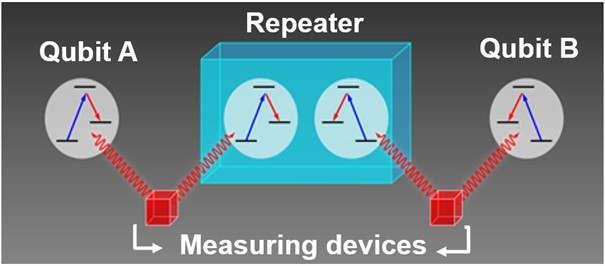
\includegraphics[width=9.2cm]{img/Memory.jpg}
		\vspace{-16pt}
		\caption{Shown here is the Quantum Repeater concept - the ``input signal" (qubit A) on the left-hand side, the ``output" signal on the right (qubit B), and the repeater states shown within the blue box. The repeater must feature two quantum states within its design, of which are entangled - shown here as the middle two states within the blue box. If each state, from left to right, is pair-entangled, then a chain of entangled states can occur. As a result, the information in the final state (qubit B) will contain information from the initial state (qubit A). The first state is entangled to the second, the second to the third, and the third to the fourth; hence the fourth state must be co-related to the first. Through this concept, the quantum signal can be repeated. Crucial to our proposal, a time-delay can be introduced to this repeater design, and thus allows for the temporary storage (memory) of qubit states.}
		\label{fig:half}
	\end{center}
\end{figure} 

\vspace{14pt}

\section{Methodology}

\begin{figure}[!tbp]
	\begin{center}
		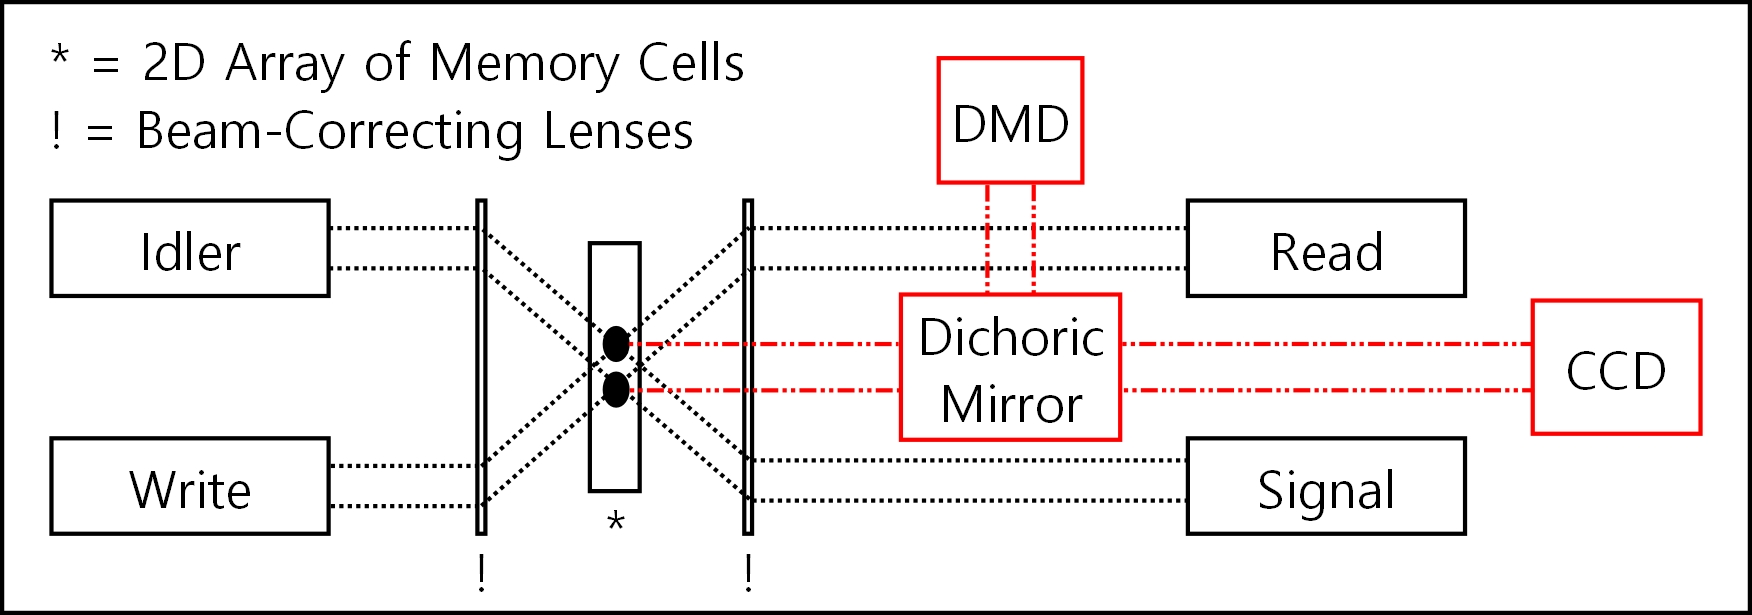
\includegraphics[width=\textwidth]{img/setup.jpg}
		\vspace{-30pt}
		\caption{A simplified block diagram depicts our proposed optical tweezers implementation, based upon the original MAQM design from C. Li et al. (2021) \citeA{MainMAQM} - a more complex diagram and explanation of the idler, signal, and read/write optical components can be found there. Highlighted in red, we show how the optical tweezers can be added to the MAQM. Two atoms (qubits) are shown in this simplified depiction, though the memory array shall be designed for a 20x20 size in the real set-up.}
		\label{fig:full}
	\end{center}
\end{figure} 

A simplified schematic of the experimental setup is shown on \ref{fig:full}. This method is proposed to improve the current state-of-the-art Multicell Atomic Quantum Memory lifespan of 1ms \citeA{MainMAQM}, up-to the increased forecast lifespan of 1s by utilising dipole traps\citeA{OptTweezer}. By modifying the setup realised by C. Li et al. (2021), replacing their MOT (Magneto-Optical Trap) with Optical Tweezers, we can contain the effects of the atomic free expansion present in the existing MAQM design\citeA{MainMAQM}.

A reservoir (not shown) is pre-loaded with evaporated Rubidium ($ \ce{^{87}Rb}$ ) atoms. The element of Rubidium is chosen as its atomic energy structure is well suited for laser cooling experiments and its vapour can be obtained at just above human body temperatures\citeA{rubidium}. The atomic ensemble is then cooled by exploiting the Doppler cooling mechanism using a pair of counter-propagating beams. Thereafter, by using M-Squared's highly tuneable SolsTiS Rainbow laser, the lasing wavelength is tuned to be much larger than that of the atomic radius of the individual Rubidium atoms within the ensemble ($ a = 248pm $) \citeA{radius}. Hence, the experiment will be taking place in the Rayleigh regime as described in the "Background" Section. 

The imaging system integrated along the optical path can digitally probe the tweezers array. This will inform us whether atoms have been trapped and for how long. An external laser acting upon the DMD - Digital Micromirror Device - allows for ultra-fast control over laser direction and atomic accessing, achieved through its digital on-off mirror switching functionality. The dichroic mirror rejects unwanted light, only allowing the passage of the correct wavelength to cancel out atomic momentum within the memory cell. Real-time information on the atomic memory cell conditions are provided through the CCD camera, though through precise timing so as to not disturb the held qubit states. Lastly, the high NA beam-correcting lenses focuses this passing light directly onto the desired atoms within the memory array. Through this process, the mitigation of atomic free expansion is achieved by removing additional momentum from each atom; thus, these atoms maintain their spatial positions for a greater time duration. 
\vspace{16pt}

\section{Timeline}

\vspace{4pt}

\begin{figure}[!htbp]
	\begin{center}
		\frame{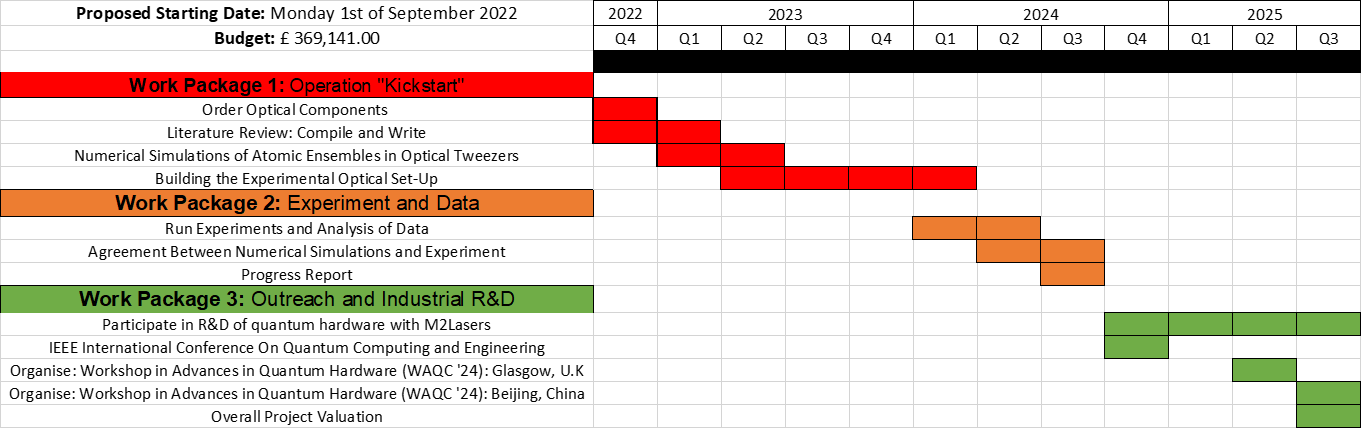
\includegraphics[width=\textwidth]{img/gantt.png}}
		\vspace{-30pt}
		\caption{Divided into yearly quarters, we have categorised our primary tasks into a three-year timeline.}
		\label{fig:full}
	\end{center}
\end{figure} 

\vspace{14pt}

\section{Finance}

A full-time Research Assistant and Co-Investigator (CI) for the complete 36 months will have a pivotal role on the project, overseeing and contributing to core lab activities daily. A laser, optics \& electronics technician (DW) working at 30\% of the full time for the first 24 months, will act as a catalyst for our research activities by overseeing and managing technicalities, and thus help with potential project delays. A secretary (MS) working at 15\% of the full time for 36 months will handle administrative tasks in order to decongest the P.I's schedule and focus on research intensive activities. Our collaborator (CL) will provide expertise on quantum repeater node hardware for the MAQM, working at 100\% of the full time for 36 months, and being paid evenly between Tsinghua University and the EPSRC. A visiting fellow (NH), employee of industrial stakeholder partner "M-Squared Lasers", will work at 100\% full-time for the last 12 months of the project (Work Package 3) and be paid by the EPSRC 30\% on fellow status (the other 70\% funded by M-Squared) - he will lead the facilitation of R\&D for scaling and commercialising the proposed qRAM.

A three-year equipment loan by Tsinghua University of the M-Squared SolsTiS Rainbow laser system is provided, which is widely tunable - compatible with our in-house laser system, for both, pre-cooling the atomic ensemble and subsequently can be utilised for the dipole traps module. Other costs for consumables and equipment required to fully realise the proposed qRAM's optical design is calculated at a rate of $\sim$ £91,500. Additionally, our numerical simulations will be run within our department's existing cluster, so no HPC related costs are forecast.

Travelling and subsistence comes in at £17,500, where the majority of the funds will go towards outreach through organising workshops on quantum hardware in the UK and China. Detailed finances of the proposal are found on the EPSRC application form.

\vspace{15pt}

\section{Outreach}
Three major conferences are planned in the third year of this project. The largest of these, the IEEE International Conference on Quantum Computing and Engineering, is where we will showcase our results and further expand our network within academia and industry. Engaging feedback and discussion here can synergise our final MAQM product offering, thus increasing our system's capability to allow external integration with other quantum systems. Having established interest from this conference, we will host two workshops in Glasgow and Beijing, focused on outreach related to scalable quantum hardware designs and encourage subsequent discussion. 

\vspace{15pt}
 
\bibliographystyleA{angew}
\bibliographyA{refs}

\end{document}